We have conducted two different experiments, one to predict the force measured
by the force sensor and another one to classify the grasp type.
The EMG data were the preprocessed as described in Sec \ref{sec:preproc}.

As said in Sec \ref{sec:adapt}, we need $N$ pre-trained models.
Then training data comes from subject $N+1$ and the system starts
training. The performace is evaluated using unseen data from the subject
$N+1$.
To simulate this scenario and to have reliable estimation of the
performance, we have used a sort of cross-validation.
In particular we consider one of the subject to generate random sequences
of training data and use the other $9$ subjects to train the stored models.
This procedure is repeated $10$ times.

To assess the performance of the proposed adaptation method we have compared it
to two baseline methods. The first one, that we call \emph{Prior}, consists in
using only the pre-trained models without updating them with the new training data.
The second one, \emph{NoAdapt}, consists in using LS-SVM using only the new data
for training, as it would be in the normal scenario without adaption.
For classification we used the classification rate as a measure of performance,
while for regression we used the correlation index because \textbf{Claudio: perche'?
hai una citazione da mettere?}.
For pre-trained models we use a standard SVM algorithm and all the parameters of the
training ($C$ and $\gamma$ of the gaussian kernel) were chosen by cross-validation.

In Figure \ref{fig:diff_cla} we have plotted the average difference between 
the classification performance of NoAdapt and our method. Using our adaptation
method there is always an improvement, but when the training samples are too
few the standard deviations are big. This is due to the high variance of the
leave-one-out error with few training samples. Still, the average gain is
almost $5\%$ when there are only 30 training samples and seems to stabilize
around $1\%$ as the training samples increase.
In Figure \ref{fig:cla_abs}.a we have plotted the best performance of our method
on a particular subject, while in Figure \ref{fig:cla_abs}.b there is the worst
performance on another subject. In the best case the gain is quite significant,
while in the worst case we almost recover the performance of NoAdapt. This is an example
where none of the models matches the new distribution of the data, so the parameter
$\beta$ is automatically set to a very small value. It is reasonable to think
that the performance of the method would increase with the number of stored
models, increasing the probability to always find a good pre-trained model.
Note that in all the cases the performance of Prior models, where well
below the performance of Adapt and NoAdapt: in Figure \ref{fig:cla_abs} is shown
only the performance of the best one among all the 9 stored models.
Similar observations can be done for the regression task in Figure \ref{fig:diff_reg}
and Figure \ref{fig:reg_abs}.

\begin{figure}[t]
  \centering
  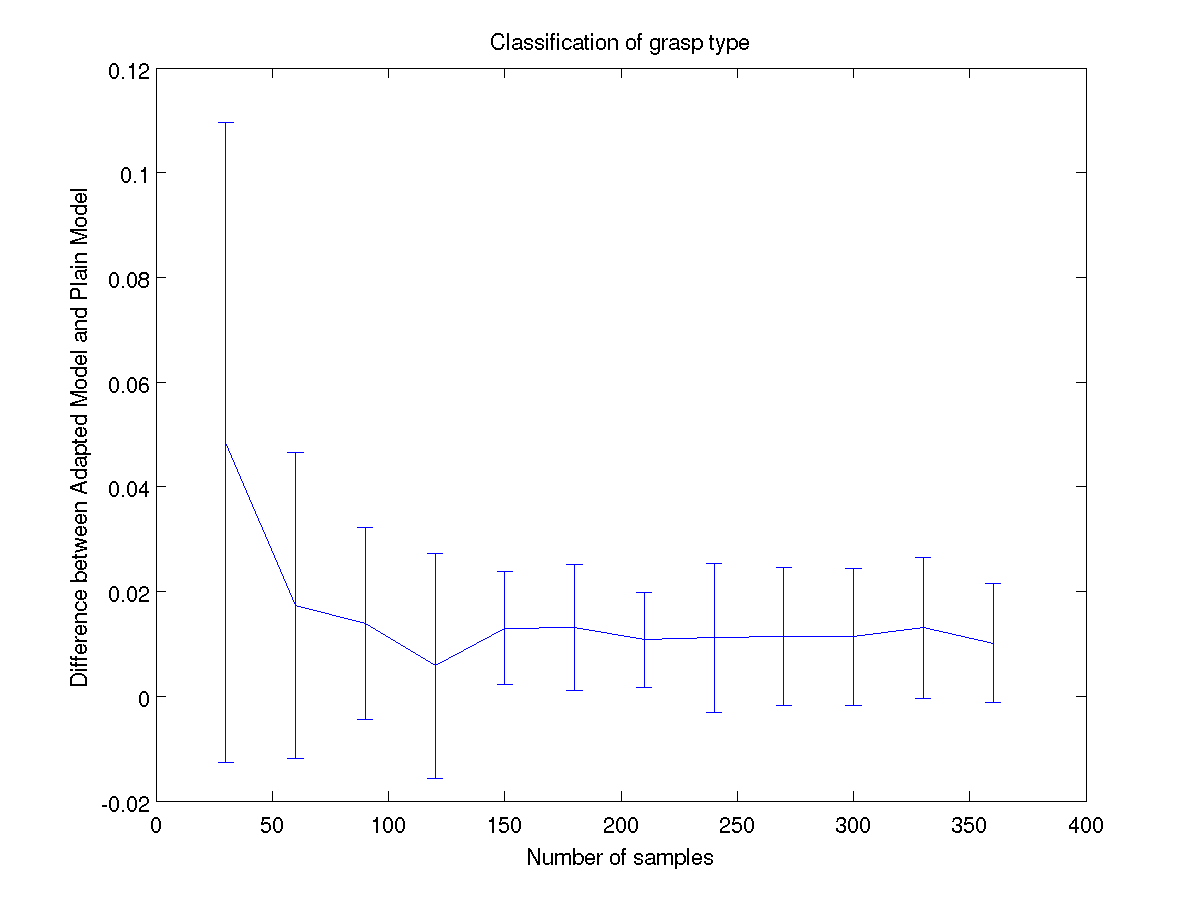
\includegraphics[width=0.95\linewidth]{figs/exp1}
  \caption{Difference in performance between NoAdapt and our method  on the
 classification of the grasp types.}
  \label{fig:diff_cla}
\end{figure}

\begin{figure*}[ht] \centering
  \begin{tabular}{cc}
    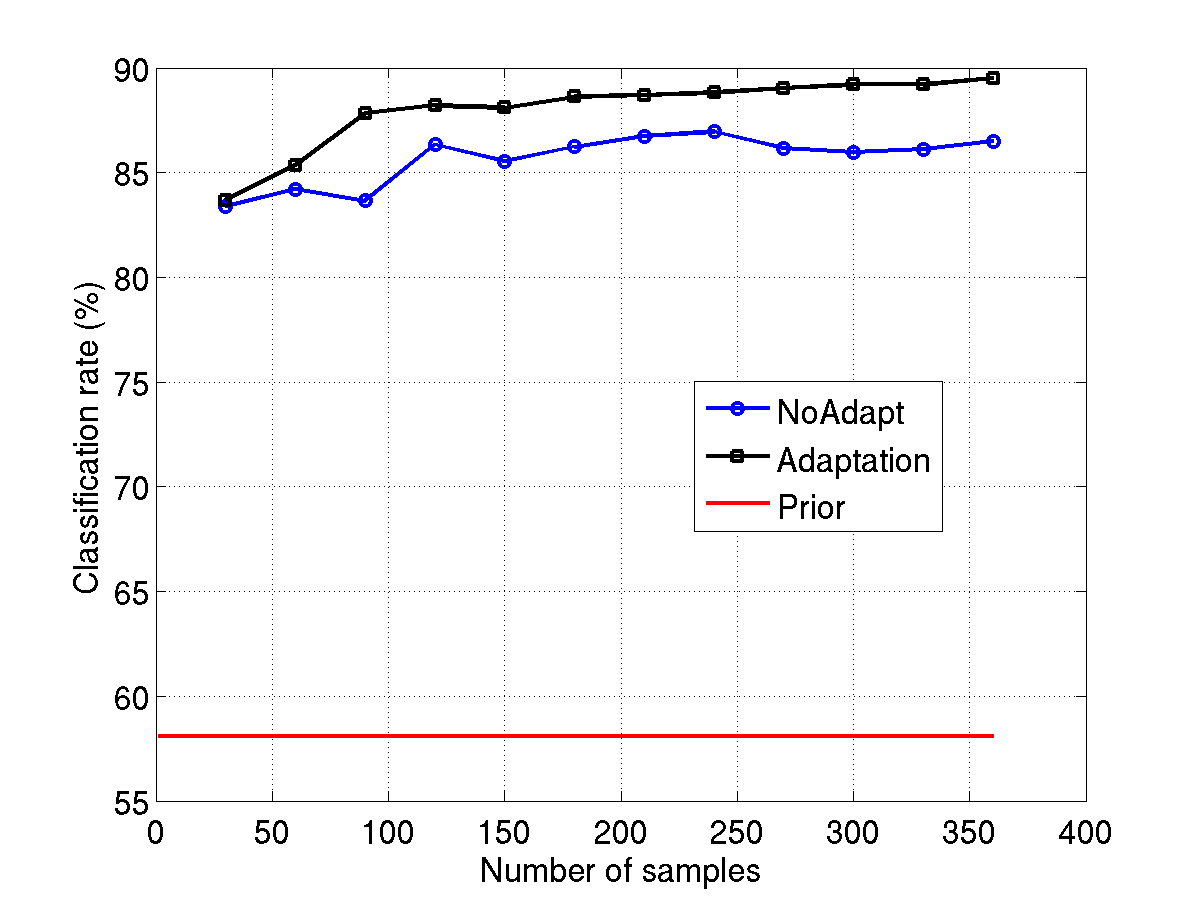
\includegraphics[width=0.45\textwidth]{figs/exp1_abs_best} &
    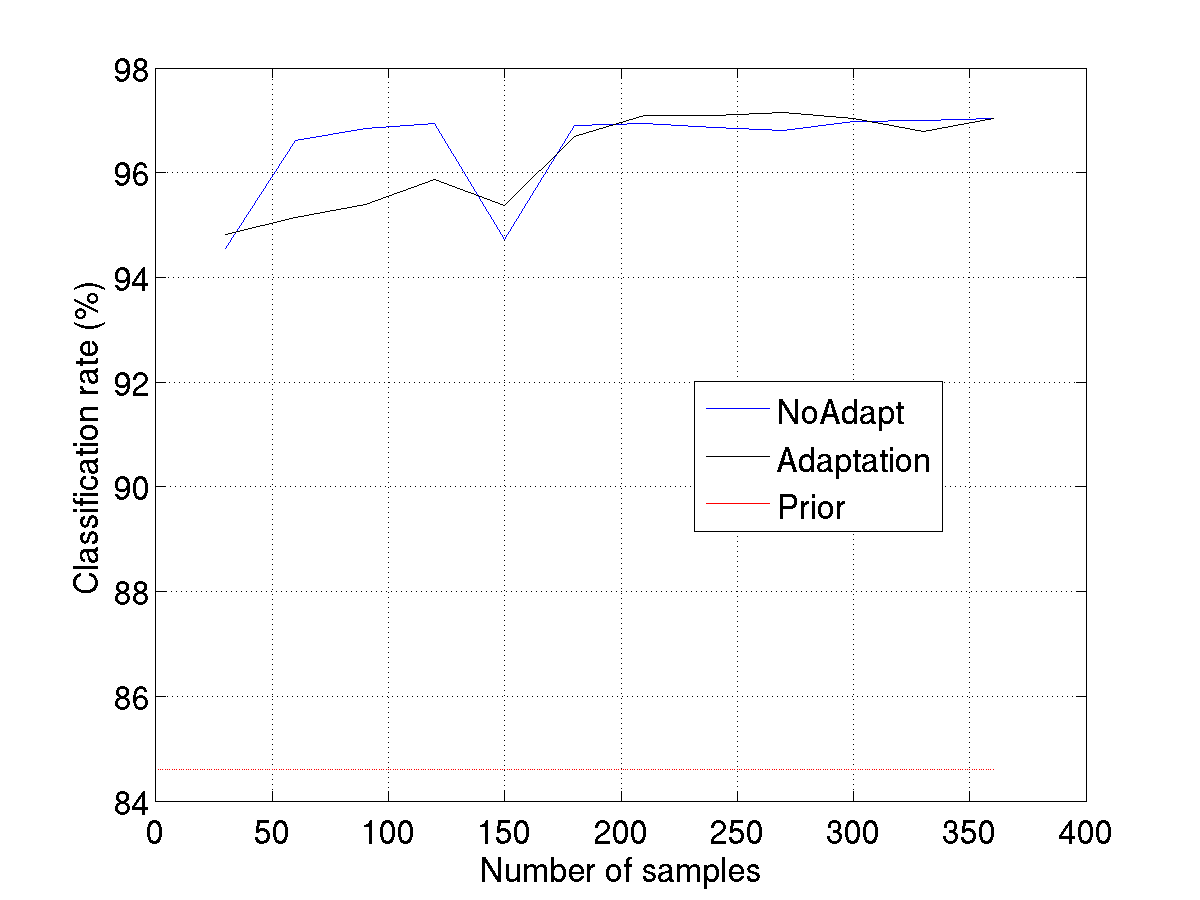
\includegraphics[width=0.45\textwidth]{figs/exp1_abs_worst} \\
    $(a)$ & $(b)$ \\
  \end{tabular}
  \caption{$(a)$ Best classification rate gain of the adapted model compared to
 NoAdapt and Prior on a particular subject; $(b)$ worst performance on another subject.}
  \label{fig:cla_abs}
\end{figure*}

\begin{figure}[ht]
  \centering
  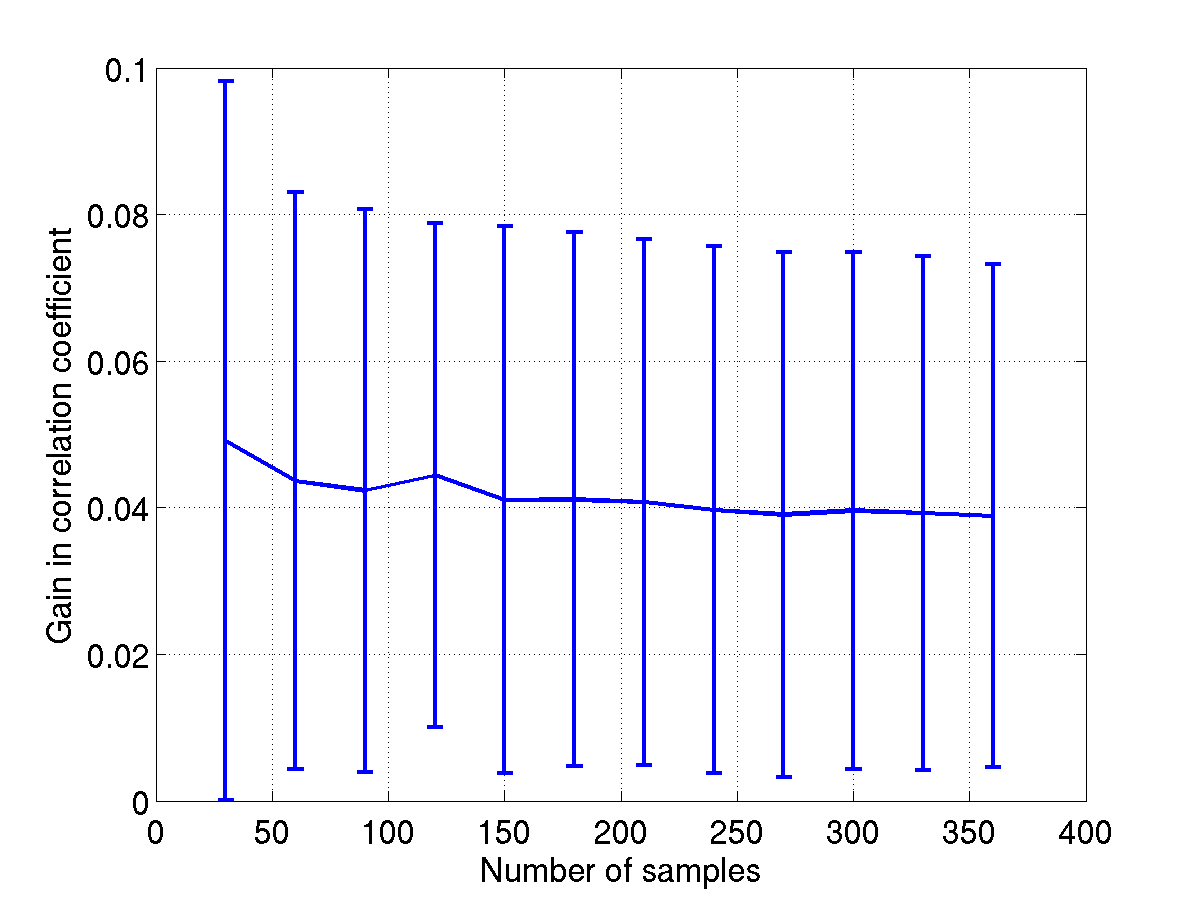
\includegraphics[width=0.95\linewidth]{figs/exp2}
  \caption{Difference in performance between NoAdapt and our method  on the
 regression of the force.}
  \label{fig:diff_reg}
\end{figure}

\begin{figure*}[ht] \centering
  \begin{tabular}{cc}
    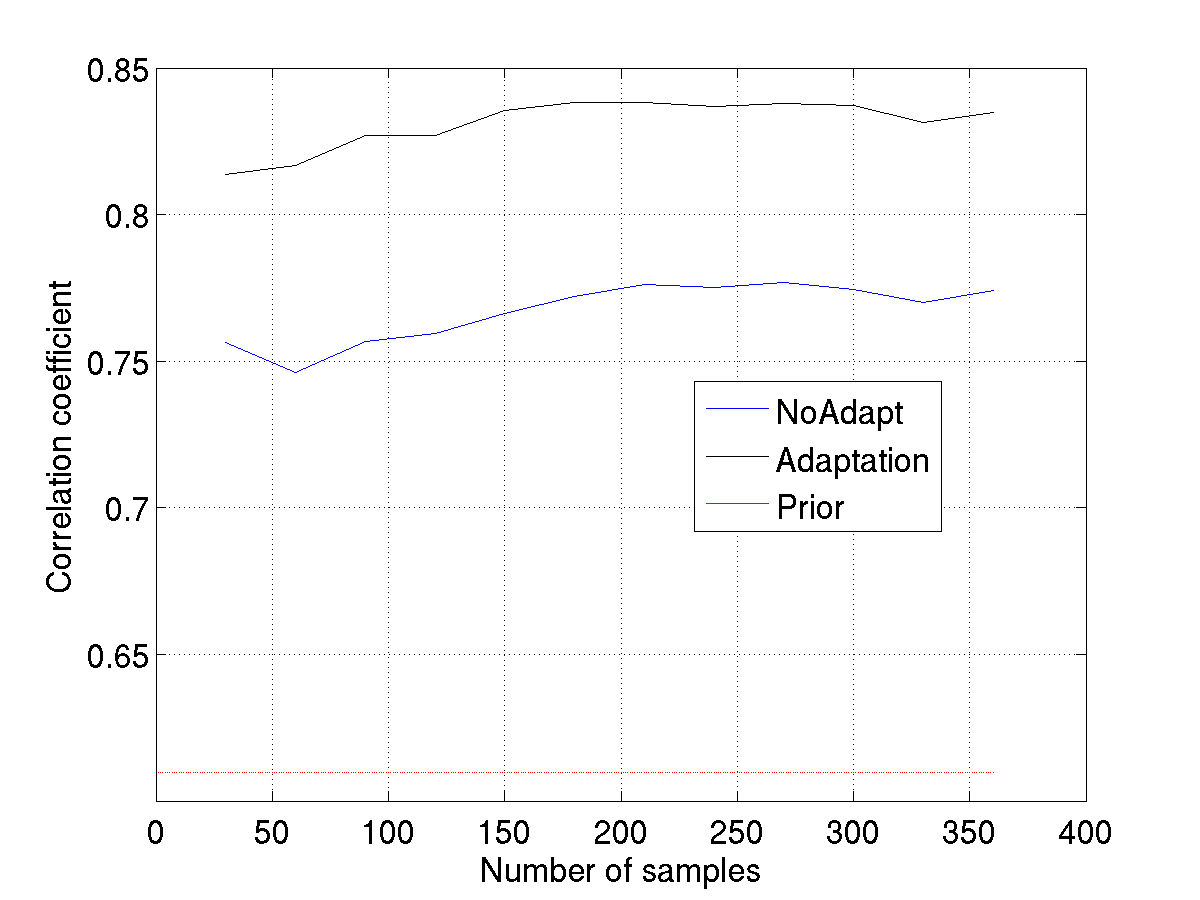
\includegraphics[width=0.45\textwidth]{figs/exp2_abs_best} &
    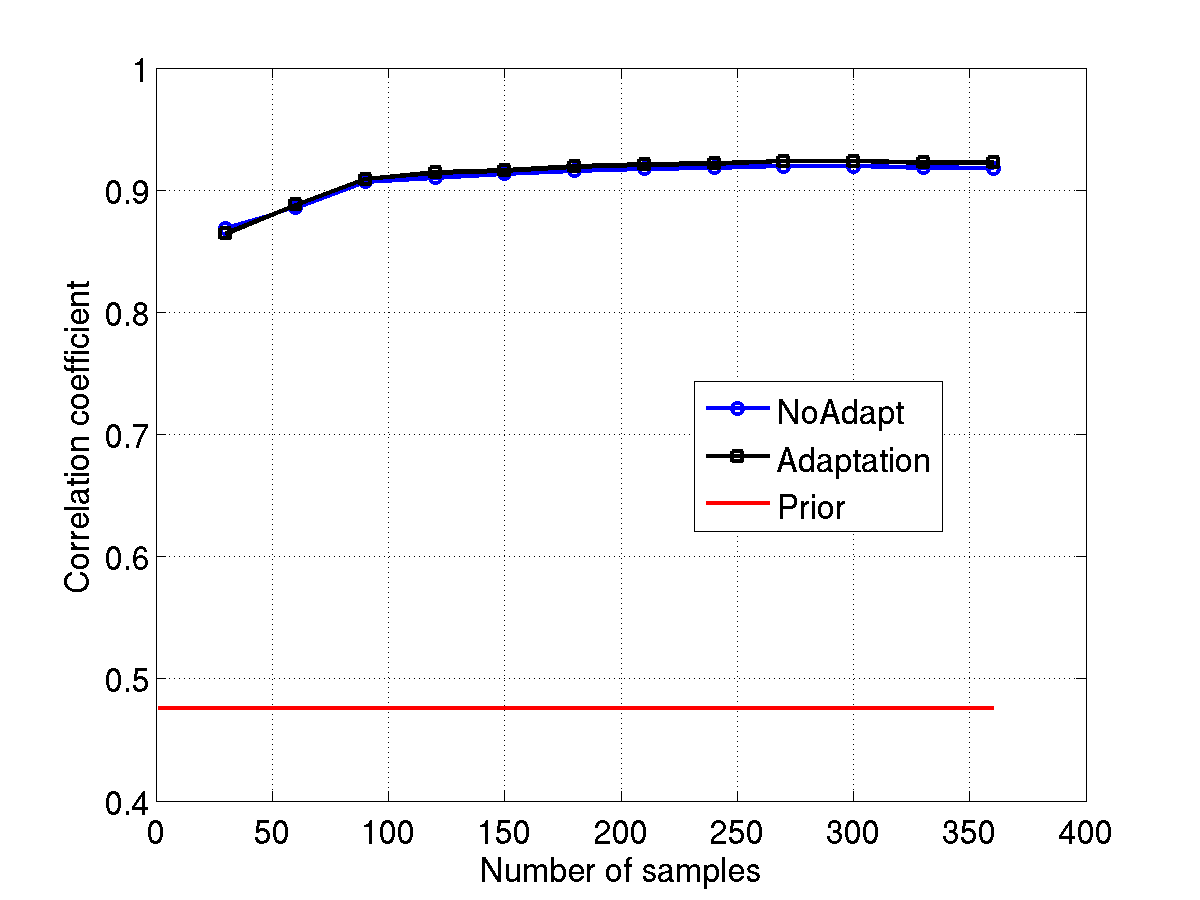
\includegraphics[width=0.45\textwidth]{figs/exp2_abs_worst} \\
    $(a)$ & $(b)$ \\
  \end{tabular}
  \caption{$(a)$ Best correlation coefficient gain of the adapted model compared to NoAdapt
 and Prior on a particular subject; $(b)$ worst performance on another subject.}
  \label{fig:reg_abs}
\end{figure*}